%
% File lfd1617.tex
%
%% Based on the style files for EACL-2017
%% Based on the style files for ACL-2016
%% Based on the style files for ACL-2015, with some improvements
%%  taken from the NAACL-2016 style
%% Based on the style files for ACL-2014, which were, in turn,
%% Based on the style files for ACL-2013, which were, in turn,
%% Based on the style files for ACL-2012, which were, in turn,
%% based on the style files for ACL-2011, which were, in turn,
%% based on the style files for ACL-2010, which were, in turn,
%% based on the style files for ACL-IJCNLP-2009, which were, in turn,
%% based on the style files for EACL-2009 and IJCNLP-2008...

%% Based on the style files for EACL 2006 by
%%e.agirre@ehu.es or Sergi.Balari@uab.es
%% and that of ACL 08 by Joakim Nivre and Noah Smith

\documentclass[11pt]{article}
\usepackage{eacl2017}
\usepackage{times}
\usepackage{url}
\usepackage{latexsym}
\usepackage{tikz}


%%%% LEAVE THIS IN
\eaclfinalcopy


\newcommand\BibTeX{B{\sc ib}\TeX}



\title{Learning from Data - Assignment 1 - Naive Bayes Classification}

\author{Remko Boschker \\
  master student of information science at the Rijks Universiteit Groningen \\
  {\tt s1282603, r.boschker@student.rug.nl} }

\date{}

\begin{document}
\maketitle
\begin{abstract}
This study compares the performance of naive Bayes, decision tree and k-nearest neighbour classification of a corpus of reviews by topic.
\end{abstract}

\section{Introduction}

This study attempts to find the best way to classify reviews by topic. I will analyse the performance of three methods and for each method I will try to find the optimal parameter settings. The methods are naive Bayes, decision tree and k-nearest neighbour classification. I will also analyse what representation of the documents gives the best performance. The representations I want to try are a vector containing the term frequency - inverse document frequency statistic for each word in the document and a sparse matrix containing per document all the counts for all the words in the corpus. For both the vectorisations I will experiment with lemmatisation of the input words and with a stop word list.

\section{Data}

The study uses a corpus of six thousand product reviews. Each review consists of a label indicating whether the review is positive or negative and a label indicating to which of the followings six topics it belongs: books, camera, dvd, health, music or software. The review also contains a file reference and the actual text of the review. The topic and sentiment labels are distributed almost equally across the corpus. About half of the reviews about a particular topic are labeled positive. Table ~\ref{tab:corpus} shows the counts for the labels in the corpus.

\begin{table}[h]\footnotesize
\label{tab:corpus}
\begin{tabular}{ l r r r r r r }
topic & cnt & \% & pos & \% & neg & \% \\
\hline
books & 993 & 16.5 & 471 & 47 & 522 & 53 \\
music & 1027 & 17.1 & 531 & 52 & 496 & 48 \\
dvd & 1012 & 16.9 & 490 & 48 & 522 & 52 \\
health & 986 & 16.4 & 470 & 48 & 516 & 52 \\
software & 994 & 16.6 & 502 & 51 & 492 & 49 \\
camera & 988 & 16.5 & 504 & 51 & 484 & 49 \\
\hline
total & 6000 & 100.0 & 2968 & 48 & 3132 & 52 \\
\end{tabular}
\caption{counts of topic and sentiment labels}
\end{table}

\section{Method/Approach}

This study compares the performance of the Scikit-learn implementations of three classification algorithms on eight different representations of the documents that need to be classified. The eight representations are generated using either the TF-IDF or Count vectoriser from the Scikit-learn Python library. Both vectorisers can be used with or without lemmatisation or the default stop word list for English included with the library. The Python NLTK toolkit performs the lemmatisation by POS tagging and then using the Wordnet Lemmatizer. I measure the performance in terms of precision, accuracy and the time it takes to train and test the models using cross-validation on one quarter of the corpus at a time.

The combinations I listed lead to a total of twenty-four experiments. I also want to improve performance by tuning the parameters of the classification algorithms. This would lead to even more combinations. I limit the number of experiments by first testing what representation works best for each of the three algorithms using the default settings and then tuning the parameters of each algorithm using the best performing representation.

\section{Optimising Representations}

\section{Tuning Classification Algorithm Parameters}

\section{Results}

\section{Discussion/Conclusion}



\section{Answers to additional questions}

\begin{enumerate}

\item decision tree theory

To build the decision tree for the given example with the least amount of nodes you need to branch on the test with the highest information gain first. Information gain is the expected reduction in entropy for the \emph{edible} label in the example for sorting on either the \emph{color}, \emph{size} or \emph{shape} labels. The information gain is calculated by calculating the entropy for the parent set and subtracting the weighted average entropy of the child sets resulting from splitting on the label. The entropy of a set is calculated by $\sum\limits_i - p_i \log_2 p_i $ where $p_i$ is the probability of an element being in class \emph{i} modeled as the portion of the elements in the set being of class \emph{i}. The information gain achieved by sorting on the \emph{colour, size or shape} features is listed in table~\ref{tab:gain}. Sorting on the \emph{size} first achieves the highest gain and therefore this is what should be done first.

\begin{table}[h]\footnotesize
\label{tab:gain}
\begin{tabular}{ l r r r r r }
& \multicolumn{4}{c}{entropy} & \\
\cline{2-5}
label & parent & child1 & child2 & avg & gain \\
\hline
colour & 0.9886 & 0.9612 & 0.9182 & 0.9531 & 0.0355 \\
size & 0.9886 & 0.8112 & 0.9544 & 0.8828 & 0.1058 \\
shape & 0.9886 & 1 & 0.8112 & 0.9528 & 0.0358 \\
\end{tabular}
\caption{information gain on the first split with respect to the edible label}
\end{table}



\begin{table}[h]\footnotesize
\label{tab:gain-small}
\begin{tabular}{ l r r r r r }
& \multicolumn{4}{c}{entropy} & \\
\cline{2-5}
label & parent & child1 & child2 & avg & gain \\
\hline
colour & 0.8112 & 0.6500 & 1 & 0.7375 & 0.0737 \\
shape & 0.8112 & 0.9182 & 0 & 0.6887 & 0.1225 \\
\end{tabular}
\caption{information gain on the \emph{small} branch with respect to the edible label}
\end{table}

\begin{table}[h]\footnotesize
\label{tab:gain-large}
\begin{tabular}{ l r r r r r }
& \multicolumn{4}{c}{entropy} & \\
\cline{2-5}
label & parent & child1 & child2 & avg & gain \\
\hline
colour & 0.9544 & 0.9852 & 0 & 0.8620 & 0.0923 \\
shape & 0.9544 & 1 & 0.9182 & 0.9387 & 0.0157 \\
\end{tabular}
\caption{information gain on the \emph{large} branch with respect to the edible label}
\end{table}

\begin{figure}
\label{fig:tree}
\caption{decision tree for predicting edible}
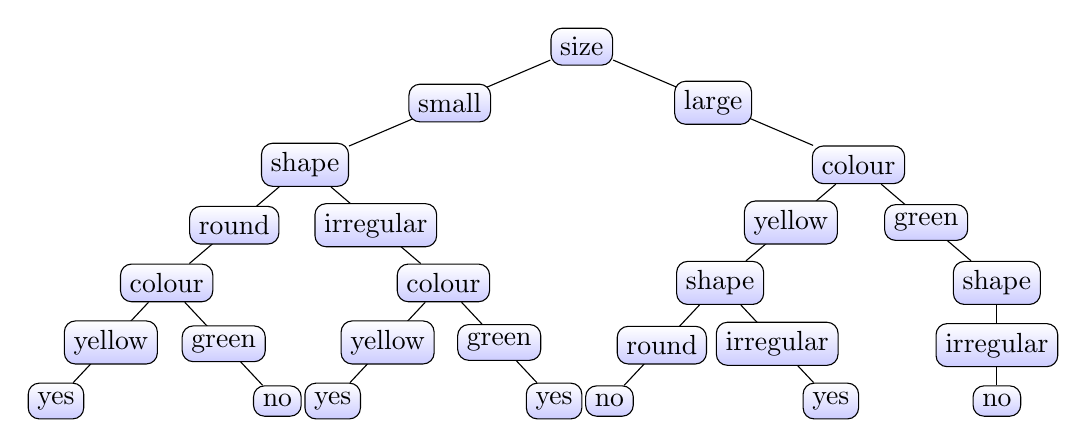
\begin{tikzpicture}[sibling distance=10em,
  every node/.style = {shape=rectangle, rounded corners,
    draw, align=center,
    top color=white, bottom color=blue!20},
  level 1/.style={sibling distance=20em},
  level 2/.style={sibling distance=10em},
  level 3/.style={sibling distance=8em},
  level 4/.style={sibling distance=8em}]
  \node {size}
    child { node {shape}
      child {node {colour}
        child {node {yes}
          edge from parent node {yellow}}
        child {node {no}
          edge from parent node {green}}
        edge from parent node {round}}
      child {node {colour}
        child {node {yes}
          edge from parent node {yellow}}
        child {node {yes}
          edge from parent node {green}}
        edge from parent node {irregular}}
      edge from parent node {small}}
    child { node {colour}
      child { node {shape}
        child { node {no}
          edge from parent node {round}}
        child { node {yes}
          edge from parent node {irregular}}
        edge from parent node {yellow}}
      child { node {shape}
        child { node {no}
          edge from parent node {irregular}}
        edge from parent node {green}}
      edge from parent node {large}};
\end{tikzpicture}
\end{figure}

As can be seen in the tables ~\ref{tab:gain-small} and ~\ref{tab:gain-large} for the items labeled \emph{small} the next split with the most gain would be by \emph{shape} and for the items labeled large it would be \emph{colour}. The resulting tree is shown in figure ~\ref{fig:tree}. The leaf for items with the features \emph{yellow,  small, round} has a $\frac{4}{5}$ probability of being edible, but a $\frac{1}{5}$ probability of not being edible. There are no features to distinguish between them. The leaf was labeled with yes, because of the higher probability. The leaf for items with the features \emph{yellow,  large, round} was treated similarly labeling such items as not edible, although there is a $\frac{1}{5}$ probability that the item is edible. There is no item with the features \emph{green, large, round} and no branch for those features is included in the tree.

\end{enumerate}

\bibliography{eacl2017}
\bibliography{yourbibfile}

\end{document}
